% Template for PLoS
% Version 3.3 June 2016
%
% % % % % % % % % % % % % % % % % % % % % %
%
% -- IMPORTANT NOTE
%
% This template contains comments intended 
% to minimize problems and delays during our production 
% process. Please follow the template instructions
% whenever possible.
%
% % % % % % % % % % % % % % % % % % % % % % % %

% Created to hold supplementary information

\documentclass[10pt,letterpaper]{article}

\usepackage[top=0.85in,left=2in,footskip=0.75in]{geometry}

% amsmath and amssymb packages, useful for mathematical formulas and symbols
\usepackage{amsmath,amssymb}

% Use adjustwidth environment to exceed column width (see example table in text)
\usepackage{changepage}

% Use Unicode characters when possible
\usepackage[utf8x]{inputenc}

% textcomp package and marvosym package for additional characters
\usepackage{textcomp,marvosym}

% cite package, to clean up citations in the main text. Do not remove.
\usepackage{cite}

% Use nameref to cite supporting information files (see Supporting Information section for more info)
\usepackage{nameref,hyperref}

% line numbers
\usepackage[right]{lineno}

% ligatures disabled
\usepackage{microtype}
\DisableLigatures[f]{encoding = *, family = * }

% color can be used to apply background shading to table cells only
\usepackage[table]{xcolor}

% array package and thick rules for tables
\usepackage{array}

% create "+" rule type for thick vertical lines
\newcolumntype{+}{!{\vrule width 2pt}}

% added by George
%\usepackage{wrapfig}
\usepackage{subcaption}


% create \thickline for thick horizontal lines of variable length
\newlength\savedwidth
\newcommand\thickcline[1]{%
  \noalign{\global\savedwidth\arrayrulewidth\global\arrayrulewidth 2pt}%
  \cline{#1}%
  \noalign{\vskip\arrayrulewidth}%
  \noalign{\global\arrayrulewidth\savedwidth}%
}

% \thickhline command for thick horizontal lines that span the table
\newcommand\thickhline{\noalign{\global\savedwidth\arrayrulewidth\global\arrayrulewidth 2pt}%
\hline
\noalign{\global\arrayrulewidth\savedwidth}}

% WATERMARKS
%\usepackage{draftwatermark}
%\SetWatermarkText{Draft}
%\SetWatermarkScale{3}

% Remove comment for double spacing
%\usepackage{setspace} 
%\doublespacing

% Text layout
\raggedright
\setlength{\parindent}{0.5cm}
\textwidth 5.25in 
\textheight 8.75in

% Bold the 'Figure #' in the caption and separate it from the title/caption with a period
% Captions will be left justified
\usepackage[aboveskip=1pt,labelfont=bf,labelsep=period,justification=raggedright,singlelinecheck=off]{caption}
\renewcommand{\figurename}{Fig}

% Use the PLoS provided BiBTeX style
\bibliographystyle{plos2015}

% Remove brackets from numbering in List of References
\makeatletter
\renewcommand{\@biblabel}[1]{\quad#1.}
\makeatother

% Leave date blank
\date{}

% Header and Footer with logo
\usepackage{lastpage,fancyhdr,graphicx}
\usepackage{epstopdf}
\pagestyle{myheadings}
\pagestyle{fancy}
\fancyhf{}
\setlength{\headheight}{27.023pt}
\lhead{
\includegraphics[width=3.0in]{PLOS-submission.eps}}
\rfoot{\thepage/\pageref{LastPage}}
\renewcommand{\footrule}{\hrule height 2pt \vspace{2mm}}
\fancyheadoffset[L]{1.25in}
\fancyfootoffset[L]{1.25in}
\lfoot{\sf PLOS}

%% Include all macros below

\newcommand{\lorem}{{\bf LOREM}}
\newcommand{\ipsum}{{\bf IPSUM}}

%% END MACROS SECTION

%% Misc. Packages
\usepackage[final]{changes}
\definechangesauthor[name={George Chacko}, color=orange]{gc}
\setremarkmarkup{(#2)}
\usepackage{listings}

\begin{document}
\vspace*{0.2in}

% Title must be 250 characters or less.
\begin{flushleft}
{\Large
\textbf\newline{Research Synergy and Drug Development: Bright Stars in Neighboring Constellations} % Please use "title case" (capitalize all terms in the title except conjunctions, prepositions, and articles).
}
\newline
% Insert author names, affiliations and corresponding author email (do not include titles, positions, or degrees).
\\
Samet Keserci\textsuperscript{1},
%Samet Keserci\textsuperscript{1,2\Yinyang},
Eric Livingston\textsuperscript{2},
Lingtian Wan\textsuperscript{1,\textcurrency},
Alexander R. Pico\textsuperscript{3},
%Name5 Surname\textsuperscript{2\ddag},
%Name6 Surname\textsuperscript{2\ddag},
 George Chacko\textsuperscript{1*}
%with the Lorem Ipsum Consortium\textsuperscript{\textpilcrow}
\\
\bigskip
\textbf{1} NETE Labs, NET ESolutions Corporation, McLean, VA, USA
\\
\textbf{2} Research Intelligence, Elsevier Inc., New York, NY, USA
\\
\textbf{3} Gladstone Institutes, San Francisco, CA, USA
\\
\bigskip


% Insert additional author notes using the symbols described below. Insert symbol callouts after author names as necessary.
% 
% Remove or comment out the author notes below if they aren't used.
%
% Primary Equal Contribution Note
%\Yinyang These authors contributed equally to this work.

% Additional Equal Contribution Note
% Also use this double-dagger symbol for special authorship notes, such as senior authorship.
%\ddag These authors also contributed equally to this work.

% Current address notes
\textcurrency Current Address: Facebook Inc., Menlo Park, CA, USA % change symbol to "\textcurrency a" if more than one current address note
% \textcurrency b Insert second current address 
% \textcurrency c Insert third current address

% Deceased author note
%\dag Deceased

% Group/Consortium Author Note
%\textpilcrow Membership list can be found in the Acknowledgments section.

% Use the asterisk to denote corresponding authorship and provide email address in note below.
*Correspondence: netelabs@nete.com
\end{flushleft}
% Please keep the abstract below 300 words
\section*{Abstract}

Drug discovery and subsequent availability of a new breakthrough therapeutic or `cure' is a compelling example of societal benefit from research advances. These advances are invariably collaborative, involving the contributions of many scientists to a discovery network in which theory and experiment are built upon. To document and understand such scientific advances, data mining of public and commercial data sources coupled with network analysis can be used as a digital methodology to assemble and analyze component events in the history of a therapeutic. This methodology is extensible beyond the history of therapeutics and its use more generally supports (i) efficiency in  exploring  the scientific history of a research advance (ii) documenting and understanding collaboration (iii) portfolio analysis, planning and optimization (iv) communication of the societal value of research.\added[id=gc,remark={expanded Abstract to state question of interest}]{ Building upon prior art, we have conducted a case study of five anti-cancer therapeutics to identify the collaborations that resulted in the successful development of these therapeutics both within and across their respecive networks.} We have linked the work of over 235,000 authors in roughly 106,000 scientific publications that capture the research crucial for the development of these five therapeutics. We have enriched the content of networks of these therapeutics by annotating them with information on research awards as well as peer review that preceded these awards. Applying retrospective citation discovery, we have identified a core set of publications cited in the networks of all five therapeutics and additional intersections in combinations of networks as well as awards from the National Institutes of Health that supported this research. Lastly, we have mapped these awards to their cognate peer review panels, identifying another layer of collaborative scientific activity that influenced the research represented in these networks. 

\linenumbers

\section*{Introduction}

Data mining of public data sources coupled with network analysis enables the quantitative description of research discoveries that were influential in the development of a breakthrough therapeutic or `cure'.  The set of scientific publications, clinical trials, patents, and regulatory approvals, linked to each other by citation or assignment, that documents the progress of concepts from basic research to a cure is termed a `cure network' \cite {bibWilliams}. Reconstructing such networks enables a deeper contextual understanding of knowledge diffusion across disciplines, scientific interests, culture, and time~\cite{bibMaldame}. Such studies also (i) provide evidence for the broad collaborative platform of basic and translational research underlying major scientific advances such as cures for diseases \cite {bibLauer} (ii) support strategic communications, and (iii) help communicate the societal value of research. The understanding of a therapeutic network, when coupled with information from clinical use of a therapeutic, also enables a recursive learning of the pathogenesis of the disease it is being used to treat, as has been noted for the burgeoning field of immunotherapeutics~\cite{bibChan}.  

Williams and colleagues have elegantly demonstrated the feasibility and value of data mining and network analysis using, as case studies, ivacaftor and ipilimumab, approved for the treatment of cystic fibrosis and melanoma respectively (\textit{vide supra}). Key assumptions in constructing these networks were that the references found in relevant documents are appropriate citations of new knowledge relevant to a given cure and that a further retrospective round of citation discovery will reveal previous influential discovery. They observed that `the nature of a cure discovery network is complex and fundamentally collaborative', noting in the case of ivacaftor, that at least 7,067 scientists with 5,666 unique affiliations contributed to ivacaftor-relevant research over a period greater than 100 years. These authors also suggest that thoughtful metrics derived from this concept could inform decision making by funders. .

 \added[id=gc,remark={clarification of question as per journal request}]{In this study, we document the collaboration networks underlying five FDA-approved therapeutics for cancer. Building upon prior art for single networks we (i) extend single network analysis to map publications and authors across multiple networks (ii) include information on research awards and peer review of grants (iii) include enriched data from a commercially available bibliographic database with disambiguated author identifiers (iv) incorporate modified network metrics and data mining methods. We observe collaboration that extends across networks and describe the role of funding and peer review in sustaining a system of layered collaborative activity in scientific discovery. By studying additional cures and research advances, we also proceed towards scaling from single case studies to mapping the entire domain of drug development with the expectation that such knowledge will be beneficial in planning, resource allocation and optimization of drug development research. We present the results of this case study as a body of work for further study by other researchers, and a step towards mapping the universe of FDA-approved drugs and biologicals.} 

\section*{Materials and Methods}  A set of five anti-cancer therapeutics, three drugs and two biologicals, approved for use in humans by the Food and Drug Administration was selected for this study (Table 1). Imatinib~\cite{bibImatinib} and Sunitinib~\cite{bibSunitinib} are tyrosine kinase inhibitors, Nelarabine~\cite{bibNelarabine} is a nucleoside analog, and Ramucirumab~\cite{bibRamucirumab} and Alemtuzumab (Campath)~\cite{bibAlemtuzumab} are humanized antibodies that target the CD52 and vEGFR-2 cell surface receptors respectively. For each of these therapeutics, a set of relevant scientific publications was constructed as in Williams et al.~\cite{bibWilliams} but with specific modifications detailed below. An allowance of 2 months was also made for `publication lag' when assembling referenced material. For example, if a therapeutic was approved on Jan 1, 2017, documents published  on or before March 31, 2017 were included. For each of the five therapeutics, a first-generation list of PubMed identifiers (citing\_pmid) was harvested from the five different data sources (Table I). 

\begin{table}[!ht]
\begin{adjustwidth}{-0.5in}{0in} % Comment out/remove adjustwidth environment if table fits in text column.
\centering
\caption{
\textbf{Case Studies of Five Anti-Cancer Agents}}
\scalebox{1}{
\begin{tabular}{|l+l|l|l|l|l|l|l|}
\hline
%\multicolumn{4}{|l|}{\bf Heading1} & \multicolumn{4}{|l|}{\bf Heading2}\\ \thickhline
Therapeutic & FDA Approval Date & Unique Identifier & US Patent & Publication Date  \\ \hline
$Alemtuzumab$ & May 2001 & BLA: 103948 & US5846534 & Dec 1998\\ \hline
$Imatinib$ & May 2001 & NDA: 021335 & US5521184 &  May 1996 \\ \hline
$Nelarabine$ & Oct 2005 & NDA: 021877 & US5424295 & Jun 1995  \\ \hline
$Ramucirumab$ & Apr 2014 & BLA: 125477 & US7498414 & Mar 2009  \\ \hline
$Sunitinib$ & Jan 2006  & NDA: 021938  & US6573293 & Jun 2003 \\ \hline
\end{tabular}}
\vspace{2.5 mm}
\begin {flushleft} Five anti-cancer therapeutics, with FDA approval dates ranging from 2001 to 2014, were selected as case studies. The unique identifier for each therapeutic is an FDA assigned NDA or BLA number. While multiple patents are typically associated with a drug or biological, the single US patent number displayed represents the primary invention that preceded approval of the therapeutic. The publication date for each patent is listed in the last column.
\end{flushleft}
\label{table1}
\end{adjustwidth}
\end{table}

\textbf{Clinical trials} The national clinical trials database (clinicaltrials.gov) was searched for clinical trials of the five therapeutics that completed by the data of FDA approval. Both cited references and publications from these clinical trials were collected if they were published within the approval date plus two months. To capture publications associated with the clinical trials that were not displayed in clinical trials.gov, PubMed was also searched with the unique identifier (NCT number) of any clinical trials that were identified. To capture publications of clinical trials not registered in clinicaltrials.gov, PubMed was searched using the therapeutic name as keyword, publication type as ``clinical trial'', and an appropriate date restriction as in searches of clinicaltrials.gov. For example, the search term (((``alemtuzumab"[Supplementary Concept] OR ``alemtuzumab"[All Fields]) OR (``alemtuzumab"[Supplementary Concept] OR ``alemtuzumab"[All Fields] OR ``campath"[All Fields])) AND (``1900/0101"[PDAT] : ``2001/07/31''[PDAT])) AND ``clinical trial"[Publication Type] was used to identify publications of clinical trials for Alemtuzumab.

\textbf{FDA documents} The drugs@fda website~\cite{bibFDA} was searched for each of the five therapeutics. \added[id=gc,remark={response to request from editor}]{Under Approval Date(s) and History, Letters, Labels, Reviews, the medical review document was copied. Cited references in the medical review document were manually extracted and matched to pmids using, as search terms in the PubMed GUI, text strings from the citation that, typically, consisted of the last name of the first author, 3-5 words of the title, the year of publication, and journal name.} FDA Approval Summaries published in journals by FDA staff, were available for all five therapeutics and contain cited references. If the published date of a cited reference in an Approval Summary exceeded the approval date plus two months, the publication was not included.

\textbf{Patents} For each therapeutic\deleted[id=gc,remark=revise for clarity]{a single patent was identified that best represented the most relevant invention to the therapeutic at hand}\added[id=gc,remark=revised]{, the original patent for the therapeutic in question was identified using a combination of web searches, Google Patents, and the scientific literature}.  
\deleted[id=gc,remark=restate]{Identification of this patent was performed using multiple web sources. The US patent number was then used to identify the patent...} \added[id=gc,remark={use example}]{For example, US5521184, the original patent for imatinib was assigned to the Ciba-Geigy Corporation in 1996 listing Zimmermann as inventor. Manual identification is assisted by a knowledge of the field}. The non-patent citation list for a patent was copied from Google Patents~\cite{bibGooglePatents} and manually processed by searching the PubMed GUI for appropriate pmids \added[id=gc,remark={response to request from editor}] {using text strings from the citation that, typically, consisted of the last name of the first author, 3-5 words of the title, the year of publication, and journal name. Returned hits were inspected for matches to the original citation in Google Patents and accepted only in the event of a high-degree of confidence in correctness} The accuracy of manual searches was far higher than a citation matching tool that we developed for this purpose and were used to generate the data in this study.

\textbf{Post-approval literature reviews} Review articles published after a therapeutic's approval by the FDA are independent studies of the the development of a therapeutic. Accordingly, PubMed was searched for review articles on these five therapeutics that were published between the date of FDA approval and a year following the date of approval. Cited references in these reviews were extracted using PubMed and Scopus. The review articles themselves were not included. 

\textbf{Pre-approval literature searches} Literature searches were performed using PubMed with a date range of 1900/01/01 to two months post-FDA approval. For example, the search term ((alemtuzumab) OR campath) AND (``1900/01/01"[Date - Publication] : ``2001/07/31"[Date - Publication]) was used to retrieve articles of interest relevant to alemtuzumab.

\textbf{PubMed and Scopus} Citing\_pmids from the five different sources above  were combined and deduplicated. Using the Scopus database and its APIs, the manually-generated list of pmids taken from the five sources mentioned (Clinical Trials, FDA Documents, Patents, Post-Approval Literature, and Pre-Approval Literature Searches) were searched in Scopus, using the basic Scopus Search API, to arrive at a list of Scopus IDs (citing\_sid) for the publications. The Scopus Abstract Retrieval API was then used to retrieve a more comprehensive record for each of the SIDs comprising that list of publications Next, for each of these publication records citing\_sid), we used the Scopus Author Retrieval API to retrieve a full record for each unique author in the  publication set. We also used the Abstract Retrieval API to collect records for each of the publications cited by the first generation of publications. This set of cited publications is the cited\_sid set.  Using the same Author Retrieval API, we then gathered data for each of the unique authors affiliated with the cited\_sid publications. Completion of the process yields two sets of publications, citing\_sid and cited\_sid, with citation links between them and full information on all authors for both generations. Finally, for each author in the study, we used the standard Scopus Search API once more to retrieve a smaller record for every publication affiliated with them in Scopus, in order to tally their overall publication output. While author records in Scopus have overall publication counts as part of the record, by manually downloading each of them, we can store and count them by type (i.e. article, book chapter, Editorial, review, etc.). This allowed us to more precisely arrive at publication totals for only those publication types that are relevant for this study. \added[id=gc,remark={clarification on network calcuation}]{For the gRBR metric (below), we counted only article and article in press when computing total researcher productivity.}

Whereas mapping between PubMed and Scopus identifiers at the citing\_pmid and citing\_sid stage resulted in 1\% or less information loss, mapping at the cited\_sid to cited\_pmid resulted in a loss of roughly 15-20 \% of target records. Accordingly the Scopus data  was used as the backbone of the publication component of the network and the cited\_pmid information was treated as an annotation layer.  These observations are summarized in Table 2. 

\begin{table}[!ht]
\begin{adjustwidth}{-0.5in}{0in} % Comment out/remove adjustwidth environment if table fits in text column.
\centering
\caption{{\bf Citation Counts and Mapping Between Bibliographic Databases}}
\scalebox{1}{
\begin{tabular}{|l+l|l|l|l|l|l|l|}
\hline
%\multicolumn{4}{|l|}{\bf Heading1} & \multicolumn{4}{|l|}{\bf Heading2}\\ \thickhline
Therapeutic & citing\_pmid count & citing\_sid count & cited\_sid count  & cited\_pmid count  \\ \hline
$Alemtuzumab$ & 599 & 587 (1\%) & 8840 (2\%) & 7071(20\%)\\ \hline
$Imatinib$ & 1380 & 1373(1\%) & 27326(1\%) &  23340(17\%) \\ \hline
$Nelarabine$ & 104 & 104(0\%) & 2476(1\%) & 1990(20\%)  \\ \hline
$Ramucirumab$ & 1820 & 1804(1\%) & 48587(0\%) & 40973(19\%)  \\ \hline
$Sunitinib$ & 1512  & 1509(0\%)  & 33895(0\%) & 28661(15\%) \\ \hline
\end{tabular}
}
\vspace{2.5 mm}
\begin{flushleft}
 Five anti-cancer therapeutics were selected as case studies. A foundational set of references (citing\_pmid) was assembled for each therapeutic from patents, clinical trials, regulatory documents, and the scientific literature (Materials and Methods). Citing\_pmids were mapped to Scopus identifiers (citing\_sid), which were used, in turn, to retrieve cited publications (cited\_sid). Cited\_sids were mapped back to PubMed identifiers (cited\_pmid).The number of  identifiers at each stage of the mapping process is shown along with percentage loss (in parentheses) when mapping across PubMed and Scopus or due to null values in the cited\_sid field.
\end{flushleft}
\label{table2}
\end{adjustwidth}
\end{table}

Both citing and cited pmids were mapped to NIH grants and peer review panels (study sections) using public information available through NIHExPORTER~~\cite{bibNIHExPORTER}. Thus, we enriched our network data by identifying those study sections associated with the awards that supported publications in our networks. 

\textbf{Networks} The resultant data were modeled as networks and analyzed using metrics based on network topology. We calculated the propagated in-degree rank (PIR) and ratio of basic rankings (RBR) metrics of Williams ~~\cite{bibWilliams}. PIR represents the sum of aggregated citation scores (first and second degree only)  for all articles in a network that can be attributed to an author. In addition to computing PIR for all authors in each network, we also combined the citation data for all five networks and computed a networkPIR (nPIR) score, which was also normalized to the sum of individual PIR scores within each network as the PIRpartitionRatio (PPR) as a way to measure inter-network influence. RBR is intended to represent the fraction of a researcher's output that is in a network and is defined as the ratio of the number of publications in network to the number of publications in a background dataset for an author. In its original specification, the background dataset for RBR was constructed by keyword searches of PubMed. A potential weakness of this keyword based approach is that keywords do not effectively capture the field or the total output of an author even if multiple background samples are taken. Therefore, we created two new variants of the RBR; network RBR (nRBR) and global-based RBR (gRBR). nRBR uses all publications in our set of five therapeutics as background and gRBR takes advantage of the Scopus author\_id to capture the total article output of an author as background. Thus, nRBR and gRBR normalize a researcher's in-network contributions to backgrounds based on total network and total researcher productivity respectively. The details of how these metrics were calculated are provided in supplementary material \nameref{S1_File}.\\

\textbf{Analysis}. All data used in this study were acquired exclusively from the sources listed above. \added[id=gc,remark={response to request from editor}]{Data used to generate the figures and tables in this study are available in a Mendeley Data repository~\cite{bibMendeley}}. Computations were performed on infrastructure owned or leased by NETE Solutions, Elsevier, or the Gladstone Institutes. Code and scripts used in this study were written in Java, Python, and R and are archived on a publicly accessible Github repository~\cite{bibGithub}. \added[id=gc,remark={details of new computing procedures}] {The publicly available codes of the Williams study~\cite{bibLotia} were used as the basis for designing the codes used in our study. The previous codes were designed to generate graph objects and make use of graph methods such as breadth-first search (BFS) and depth-first search (DFS for graph traversal. In our approach, we used basic data structures like hash maps, hash sets, lists and aggregations and enriched the first generation set of references with data from Scopus, which indexes more scientific journals~\cite{bibFalagas}, cited references from post-approval literature reviews, cited references from FDA Approval Summaries, direct PubMed searches, grants and peer review data. In the Williams study, assembly and analysis of each network took roughly 17 hours per drug, 10 of which are manual processing steps. While our process also involved expert level curation of a foundational set of references for each drug with a cost of roughly 2-5 hours, our network calculations and metrics ran in the order of minutes once the bibliometric data were assembled.} Network visualization was performed using Cytoscape~\cite{bibCytoscape}.}

\section*{Results and Discussion} 
\textbf{Publications} Scientific publications form the backbone of each of these five networks. Our initial assumptions of appropriate citation and retrospective citation discovery (Introduction) suggest that network nodes that are common to multiple networks are likely to be influential. We calculated intersection counts for all possible combinations of publications in the Alemtuzumab, Imatinib, Nelarabine, Ramucirumab, and Sunitinib networks (\nameref{S2_Table 1}). We also applied intersection analysis at a finer level of granularity by computing intersection counts for both first generation citations (citing\_pmid) and second generation citations (cited\_sid). The results are displayed as Venn diagrams in Fig. 1. 

\begin{figure}[!h]
%\begin{adjustwidth}{-0.5in}{0in} % Comment out/remove adjustwidth environment if table fits in text column.
\centering
\scalebox{0.99}
{
\begin{subfigure}{.5\textwidth}
  \centering
%  \includegraphics[width=.95\linewidth]{}
  \label{fig:sub1}
\end{subfigure}
\begin{subfigure}{.5\textwidth}
  \centering
 % \includegraphics[width=.95\linewidth]{}
  \label{fig:sub2}
\end{subfigure}
}
\caption{{\bf Intersecting Publications in Five Networks} Intersections were calculated across all five networks for the first generation of references (citing\_pmids) and 
as well as for the second generation of references (cited\_sids) and displayed as Venn diagrams.  \emph{Left Panel.} No first generation publications are observed common to all five networks. A single publication is cited in four of five networks. \emph{Right Panel.} 14  publications are common to all five networks. Abbreviations: alem (Alemtuzumab), imat (Imatinib), nela (Nelarabine), ramu (Ramucirumab), suni(Sunitinib)}
\label{fig: test}
%\end{adjustwidth}
\end{figure}


The intersection of all five networks consists of 14 publications out of a total of 106,720 unique Scopus identifiers. Strikingly, not even a single publication is common to all five networks at the first generation level (citing\_sid) although a single publication, the pathbreaking work of Kohler and Milstein on the production of monoclonal antibodies~\cite{bibKohler}, is cited in four out of five networks. All 14 publications are in the second generation of citations (cited\_sid) and another 198 comprise the sum of intersections in all possible four-network combinations, roughly an order of magnitude greater than the case of cited references. We manually grouped these 14 publications using high level descriptive terms and observed that this group was composed of  statistical methods (5 publications), molecular and cell biological methods (4 publications), analytical and structural biology techniques (3 publications) and cancer biology (2 publications). Of these last two, one is a review of the p53 gene~\cite{bibLevine} and the second is a study of angiogenesis in children with acute lymphoblastic leukemia~\cite{bibFolkman}. Thus, the majority of this small set of 14 publications describes methods that are heavily cited in these therapeutic development networks, which is consistent with observations of the general scientific literature ~\cite{bibVanNoorden}. The relationship between core publications and their therapeutic networks is visualized in Fig. 2. As the subject of another study, we are actively working on a scalable automated strategy to characterize the entire dataset as well as all combinations of intersections between networks using high level descriptive terms.

\begin{figure}[!h]
%\begin{adjustwidth}{-0.5in}{0in} % Comment out/remove adjustwidth environment if table fits in text column.
\centering
%\scalebox{1.3}{
%\includegraphics[scale=0.1]{cy_core14_v2csv_5b.png}}
\caption{{\bf Core Publications in Networks}  The outer arcs of blue nodes identifies first generation publications (citing\_sid) for each therapeutic. Nodes in the inner ring are sized by a gradient proportion to total degree count with an upper limit of 30 and are colored by a gradient proportional to the number of drug connections (2 to 5). 14  publications are common to all five networks (Table 3) and are colored red. The remaining nodes in the inner ring connect to between 2 and 4 drugs each and are labeled accordingly. Abbreviations: alem (Alemtuzumab), imat (Imatinib), nela (Nelarabine), ramu (Ramucirumab), suni(Sunitinib).}
\label{fig2}
%\end{adjustwidth}
\end{figure}

\textbf{Grant Support} With its annual budget of approximately US\$32 billion, NIH is a major funder of biomedical research through its granting program. Understanding the nature and extent of NIH grant support for the research represented in our five networks, provides insight into the funding programs that enabled this research. We took advantage of publicly available data~\cite{bibNIHExPORTER} to identify grant support for the publications in our five networks by mapping them to pmids. A total 19,104 unique grant numbers was harvested of which 112 were found in all five networks. At the intersection of five networks, the reason the number of grants is larger than the number of publications is because publications and grants exist in a `many to many' relationship in that each publication can acknowledge support from multiple grants and each grant can support multiple publications. These awards were grouped by major type  and visualized (Fig 3.). Of note, support from Research Program Projects and Center grants is proportionately larger in the intersection group when compared to the total population where the proportion of research projects is larger. A significant loss of information occurs when mapping from cited\_sid to cited\_pmid (Table 2). Thus we believe that these numbers may be an underestimate of actual grant support from NIH. Also missing from this analysis are details of research support from other funding agencies and industry, which are questions that we intend to pursue. Even so, these data testify to a recurring theme of collaboration and breadth of community engagement that is also seen at the publication level. We speculate that the broader and collaborative nature of such awards may be more likely to result in a methods-rich population of publications than the more focused research project award but elucidation will require further and more rigorous study. 

\begin{figure}[!h]
%\begin{adjustwidth}{-0.5in}{0in} % Comment out/remove adjustwidth environment if table fits in text column.
\centering
%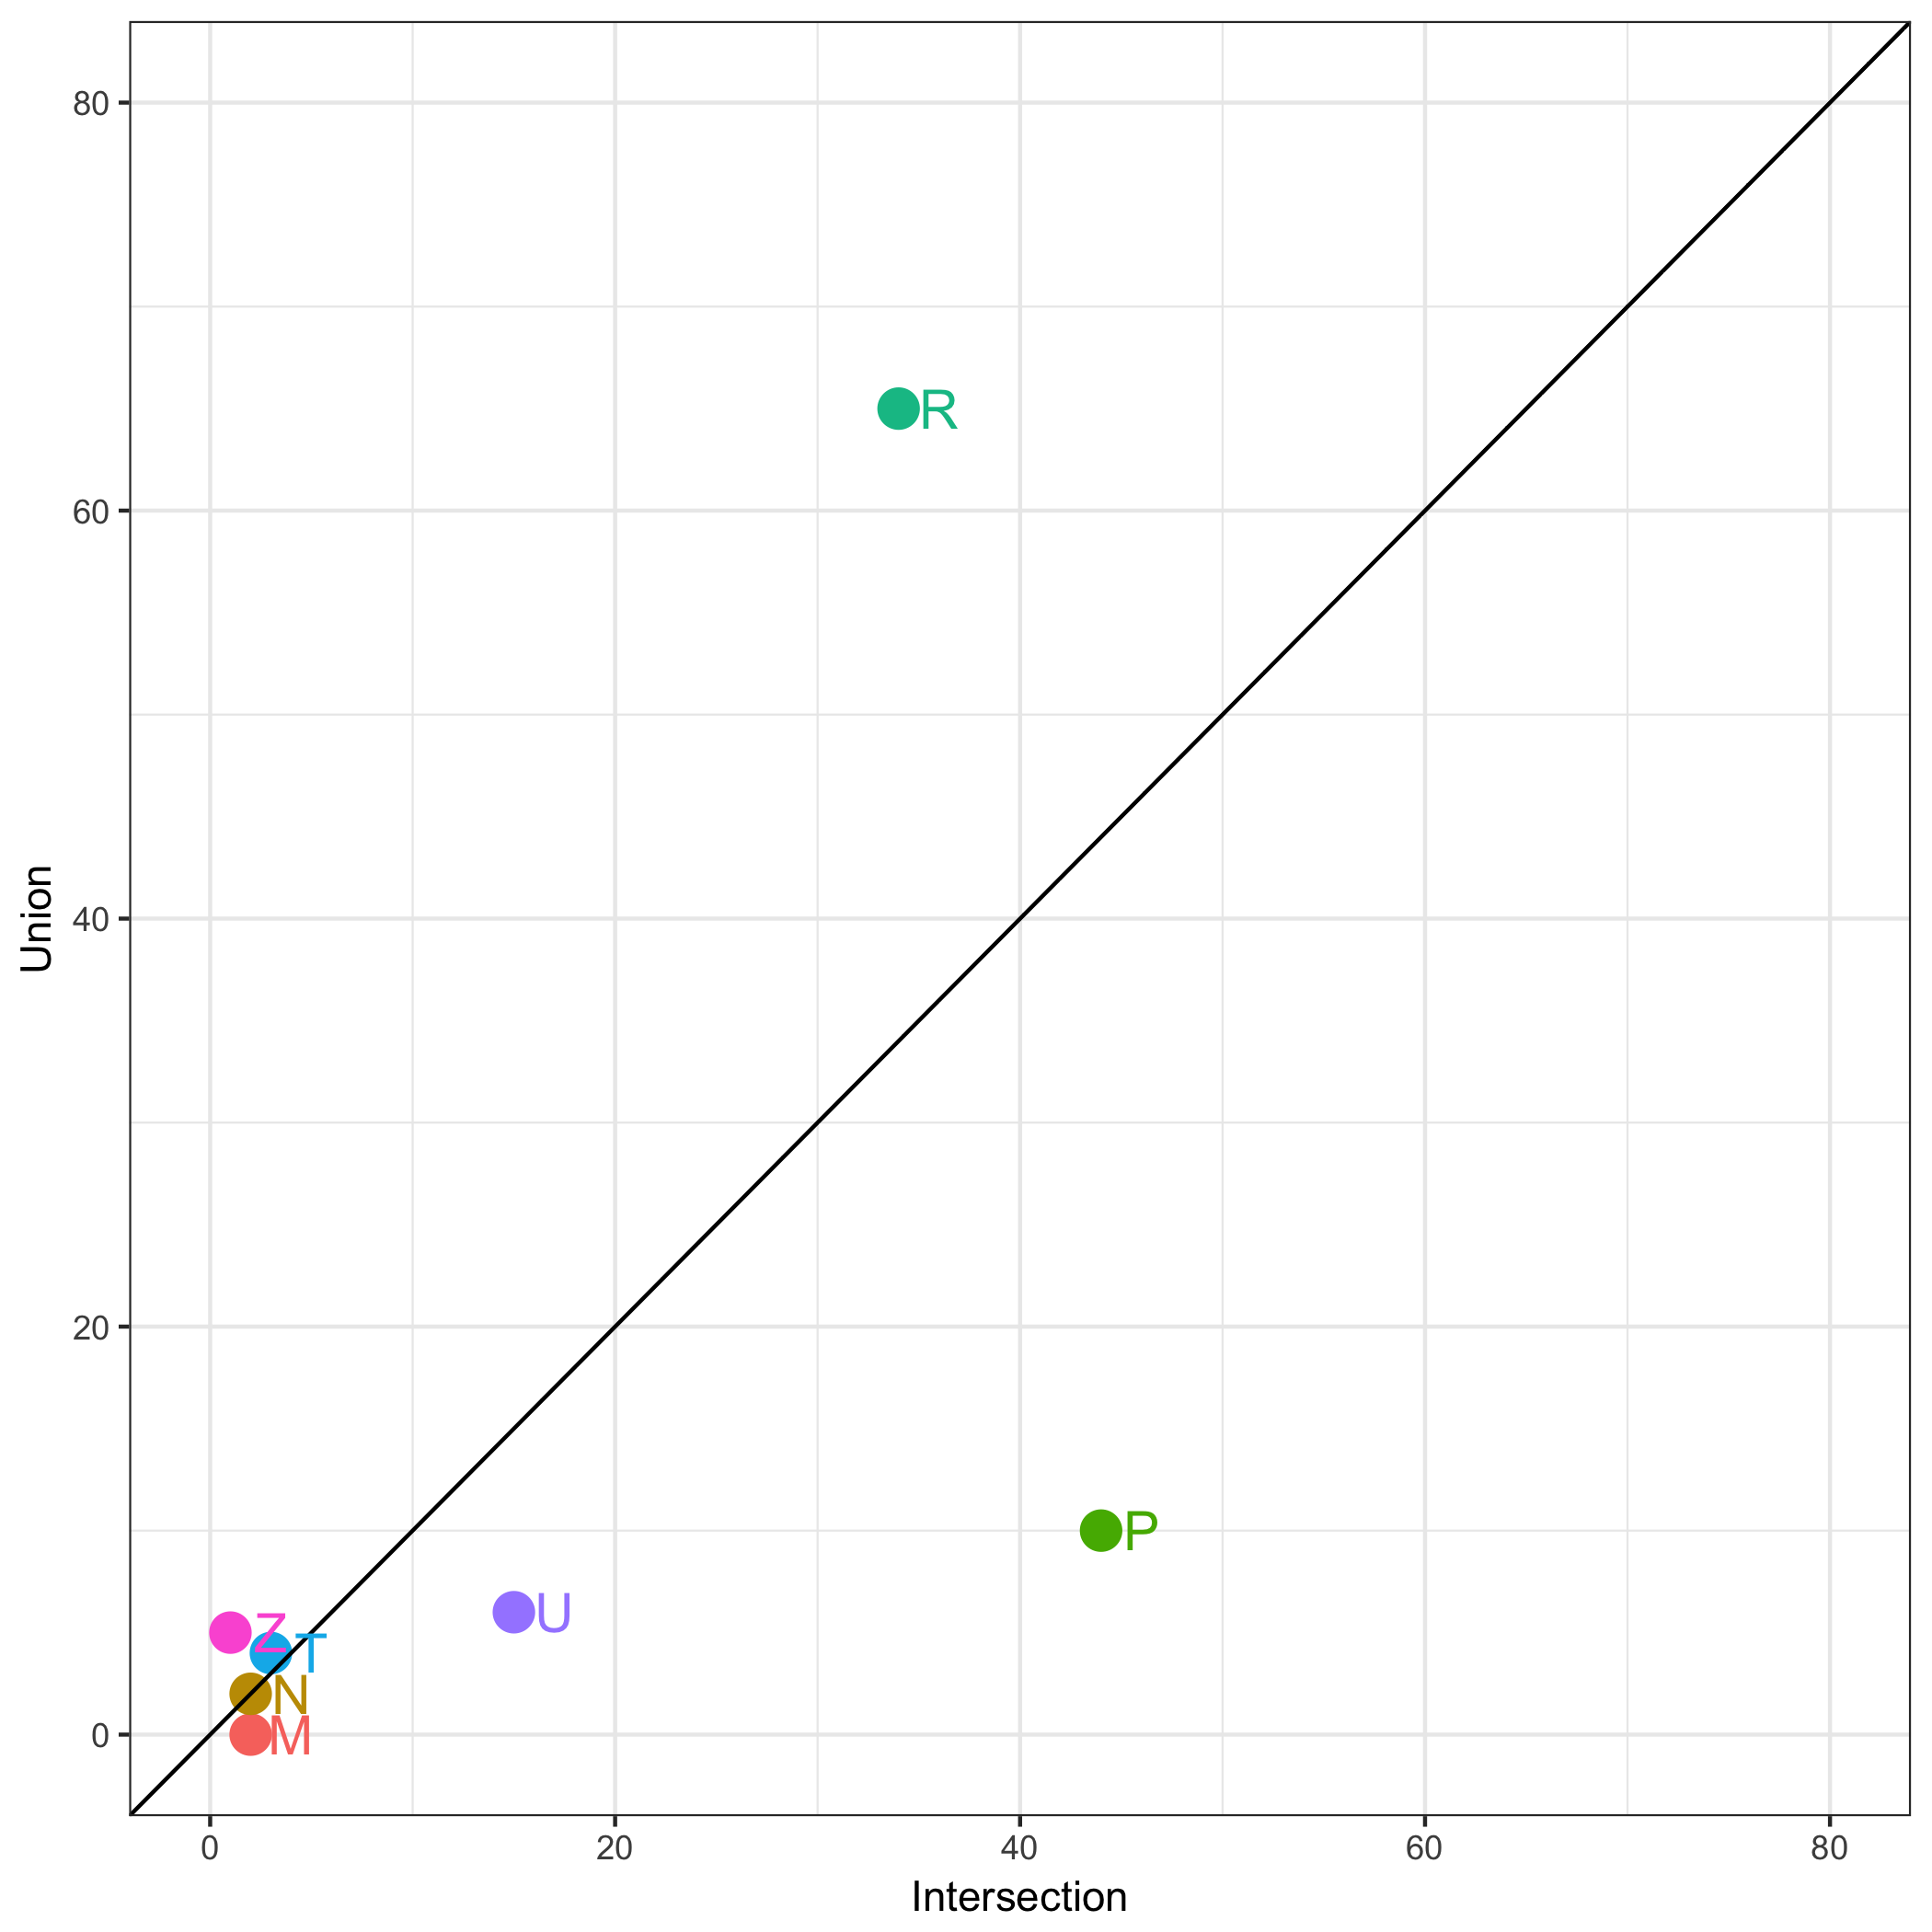
\includegraphics[scale=0.1]{proj_percent.png}
\caption{{\bf NIH Research Support} Grant and contract support for publications from NIH in the five networks was identified using ExPORTER data (Materials and Methods). 19,104 unique project numbers were identified as sources of support for publications in all five networks. Of these, 112 projects were common to all five networks. Projects were grouped by mechanism (i) P-  Research Program Projects and Centers (ii) R- Research Projects (iii) M-General Clinical Research Centers Programs (iv) N-Research and Development-Related Contracts (v) U-Cooperative Agreements (vi) T-Training Programs (vii) Z- Intramural Research. For each mechanism, the number of projects in the intersection of all five networks was plotted against the number in the union of all five networks (both expressed as percentages of their respective totals). A higher proportion of Research Program Projects and Centers awards is found in the intersection group.}
\label{fig3}
%\end{adjustwidth}
\end{figure}

\textbf{Peer Review} Research support from NIH is typically made through a two stage peer-review process.  The Center for Scientific Review at NIH manages first-stage scientific review of between 50,000-60,000 grant applications each year~\cite{bibBoyack}, a process involving more than 15,000 expert reviewers. In addition, individual Institutes and Centers at NIH manage smaller scale peer review operations. Considering a crude estimate of a 20\% success rate in funding, peer review can be viewed as a collaborative scientific activity and that serves as a selection layer for the upper fifth of applications, thus strongly influencing granting outcomes. To describe this layer at a high-level, we matched the awards in the the five networks to the peer review panels (study sections) that evaluated them for scientific merit and calculated the intersection and union of these peer review panels. Eighty eight unique panel identifiers formed the intersection. Of these, 11 are distinguishable as Special Emphasis Panels that could be either one-time or recurring panels with temporary members, the remaining 77 are chartered panels with relatively stable membership. Some of these panels are no longer active and public records are not easily available to determine their scientific focus. For the 74 panels that could be classified (Supplemental), beyond an obvious focus on cancer, it is evident that the panels represent a rich mix of disciplines such as chemistry, biophysics, genetics, cell biology, and molecular biology; as well as AIDS, pathology, radiology, endocrinology, neurology, mental health, and child health. Four hundred and seven unique panel identifiers formed the union of all five networks. Of these 28 were Special Emphasis Panels, the remaining 379 panels were chartered as in the case of the intersection. These data provide evidence of broad input from invited experts in a collaborative activity that selects promising scientific projects. Assuming an average of 25 reviewers per panel (the number is likely to range from 5-40) and excluding that some of these panels are likely to have met multiple times during the lifespan of the awards in question and that some of these applications for funding may have been reviewed multiple times, a minimum of 10,000 experts comprised this additional layer of scientific influence. We believe that the actual number is likely to be at least double. A more accurate estimate would be possible if historical records of participation in peer review were made publicly available by NIH. We do not have records of funding awards or peer review from sources other than NIH and this is a focus of future investigation.

\textbf{Network Metrics}  \added[id=gc,remark={revise discussion of methodological advances}]{We have built upon the work of Williams~\cite{bibWilliams} by addressing author disambiguation through the use of Scopus authorIDs and enriching the network data with grants and peer review data. Whereas, the original code was designed to handle a single drug and was not applied to a problem larger than 5000 articles, our approach scales to over 100,000 articles and our metrics include cross-network calculations.To quantify network data and to identify influential researchers in and across networks, we calculated PIR and RBR scores for all researchers as well as the new nPIR, PPR, nRBR, and gRBR scores (Materials and Methods, Supplemental Information). The nPIR metric describes the sum of aggregated citation scores for all articles that a researcher has in all five networks. The PIRpartitionRatio (PPR) normalizes the nPIR metric for an researcher to the sum of the researcher's individual PIR scores for each network being studied. A limitation of the nPIR and nRBR measurements is that they are valid only for the network(s) being studied. Scaling from five to the more than 1400 drugs approved by the FDA (and their many variants) would address this limitation~\cite{bibKinch}, although other data related issues may well emerge.} 

While theoretically appealing (Materials and Methods), the gRBR is the most sensitive to data quality since it relies on an accurate estimate of total productivity of a researcher, which in turn depends on data quality in bibliometric databases. We found several instances in the top 10\% of PIR scores where the gRBR was implausible likely on account of polysemy, synonymy, or incompleteness. This metric is therefore likely to be useful when the author disambiguation problem and article capture is resolved to the point where data quality is significantly improved and is not recommended except when strong confidence exists in the total productivity counts. These metrics may be best used in conjunction with positional measures such as quantiles to define populations of researchers within related networks, e.g, the top 25 researchers based on nPIR scores of all researchers in our dataset (\nameref{S3_Table 2}).  These `bright stars' are elite performers in network(s) of clinical and basic science researchers that reinforce the concept of collaborative translational achievements built upon a body of basic science. Beyond simple aggregation, weighting, and normalization that we have used, a variety of citation metrics such as SNIP~\cite{bibWaltman}, with different normalization strategies at the field, journal, and article level are available for impact analysis and these could be applied to such networks depending on the features of these networks and the aim of the study~\cite{bibIoannidis}. The use of these citation measures will assume greater importance with scale up from small numbers of networks to a greater proportion of the global research network.

\added[id=gc,remark={expanded discussion of generalizability as per editor request}]{In this study, we begin with the literature directly cited in the approval process for five therapeutics. The approval process for therapeutics is subject to multiple layers of independent assessment, i.e., patent awards, clinical trials, and FDA reviews, each of which cite relevant literature. However, the only requirement of the current method is a starting set of articles. The method is applicable to any other therapeutic or set of therapeutics, but also to medical devices, diagnostics, standards development, and research discoveries and protocols such as induced pluripotent stem (iPS) cells~\cite{bibIPS}  or CRISPR-Cas9~\cite{bibCRISPR}. Thus, any question premised upon accessible citation records and defined by a nucleus of articles can be addressed with our approach. Furthermore, the method is also generalizable to sets of articles defined by groups of authors (e.g., consortia, programs), by institutions or departments, or by grant portfolios. The application of our method to the bibliographic record of a department, for example, would provide novel, network-based metrics by which to assess collaboration, productivity, and translational impact. No matter the application, the method is implicitly time-dependent, allowing one to make historical comparisons and to set future goals. Importantly, our improvements to the method as presented here allow for the analysis across sets of articles in addition to within, supporting higher level interrogations of the crosstalk and collaborations that connect groups.}

In summary, we have demonstrated a digital methodology based on data mining and network analysis, not restricted to  drug discovery and cures alone, that offers burden-reduction in explorations of science history. Beyond assembling a set of facts about a major scientific advance, it contributes to the understanding of collaboration across domains and can be used to  enrich portfolio analysis, planning and optimization, as well as communications of the societal value of research. The approach can be easily adapted to study the collaborative history within and across research portfolios of groups of researchers and targeted programs. \deleted[id=gc,remark={delete in view of previous paragraph}]{such as the Clinical and Translational Science Award (CTSA) Program.} While finer critical evaluation of the content of datasets generated through this approach is best left to experts, the methodology is broadly accessible and can be viewed as another tool for citizen science. Overall, no single metric will provide very useful answers, instead expert interpretation of multiple metrics best matched to curated datasets will be of value.

\nolinenumbers
 
\section*{Acknowledgments} This study would not have been possible without data that is made publicly available by NIH and the FDA. We thank Tandy Warnow from the University of Illinois Urbana-Champaign for critical comments and advice on formalizing definitions. We also thank Sandeep Somaiya from NETE and Holly J. Falk-Krzesinski, Daniel Calto, M'hamed Aisati, and Sherif El Shamy from Elsevier for their support of this collaboration.
 
\begin{thebibliography}{10}

\bibitem{bibWilliams}
Williams RS, Lotia S, Holloway AK, Pico AR.
\newblock {{F}rom Scientific Discovery to Cures: Bright Stars within a Galaxy.}
\newblock Cell. 2015 163:21--23.

\bibitem{bibMaldame}
Maldame J.
\newblock {{T}he Importance Of The History Of Science In Intellectual Formation.}
\newblock Scripta Varia 2002 104:237-248.

\bibitem{bibLauer}
Lauer MS.
\newblock {{P}CSK9 Inhibitors: Lots of Work Done, Lots More to Do.}
\newblock Ann Intern Med. 2016 164(9):624-625.

\bibitem{bibChan}
O'Shea JJ, Kanno, Y., Chan AC.
\newblock {{I}n Search of Magic Bullets: The Golden Age of Immunotherapeutics.}
\newblock Cell. 2014 157:227-240.

\bibitem{bibImatinib}
Buchdunger E, Zimmermann J, Mett H, Meyer T, M\"uller M, Druker BJ, Lydon NB.
\newblock {{I}nhibition of the Abl protein-tyrosine kinase in vitro and in vivo by a 2-phenylaminopyrimidine derivative.}
\newblock Cancer Res. 1996 56(1):100-4

\bibitem{bibSunitinib}
O'Farrell AM, Abrams TJ, Yuen HA, Ngai TJ, Louie SG, Yee KW, et al. 
\newblock {{S}U11248 is a novel FLT3 tyrosine kinase inhibitor with potent activity in vitro and in vivo.}
\newblock Blood. 2003 101(9):3597-605.

\bibitem{bibNelarabine}
Ho PT, Cheson BD, Phillips PH.
\newblock {{C}linical trials referral resource. Clinical trials using compound 506U78.}
\newblock Oncology (Williston Park). 1996 10(12):1831-2.

\bibitem{bibRamucirumab}
Krupitskaya Y, Wakelee HA.
\newblock {{R}amucirumab, a fully human mAb to the transmembrane signaling tyrosine kinase VEGFR-2 for the potential treatment of cancer.}
\newblock Curr Opin Investig Drugs. 2009 10(6):597-605.

\bibitem{bibAlemtuzumab}
Hale G, Bright S, Chumbley G, Hoang T, Metcalf D, Munro AJ, Waldmann H.
\newblock {{R}emoval of T cells from bone marrow for transplantation: a monoclonal antilymphocyte antibody that fixes human complement.}
\newblock Blood. 1983 62(4):873-82.

\bibitem{bibFDA}
Federal Drug Administration.
\newblock {{D}rugs@FDA: FDA Approved Drug Products.}
\newblock https://www.accessdata.fda.gov/scripts/cder/daf/.

\bibitem{bibGooglePatents}
Google Inc.
\newblock {{G}oogle Patents}
\newblock https://patents.google.com/.

\bibitem{bibNIHExPORTER}
National Institutes of Health.
\newblock {{N}IH ExPORTER}
\newblock https://exporter.nih.gov/.

\bibitem{bibMendeley}
Keserci S, Livingston, E, Wan  Lingtian, Pico A, Chacko, G.
\newblock {{B}right Stars in Neighboring Constellations v4.}
\newblock Mendeley Data http://dx.doi.org/10.17632/ysh53v7gpz.4

\bibitem{bibFalagas}
Falagas ME, Pitsouni EI, Malietzis GA, Pappas G.
\newblock{{C}omparison of PubMed, Scopus, Web of Science, and Google Scholar: strengths and weaknesses.}
\newblock FASEB J. 2008 22(2):338-42. 

\bibitem{bibGithub}
Keserci S, Livingston E, Wan L, Pico AR, Chacko G.
\newblock {{N}ET ESolutions, NETE Labs}
\newblock https://github.com/NETESOLUTIONS/NETELabs\_CaseStudies/tree/master/Bright\_Stars.

\bibitem{bibLotia}
Lotia, S., and Pico, A.P. 
\newblock {{Gladstone Bibliometrics}
\newblock https://github.com/ gladstone-institutes/bibliometrics/tree/1.0.1.

\bibitem{bibCytoscape}
Shannon P, Markiel A, Ozier O, Baliga N, Wang JT, Ramage D, et al.
\newblock {{C}ytoscape: a software environment for integrated models of biomolecular interaction networks.}
\newblock Genome Res. 2003 13(11):2498-504.

\bibitem{bibKohler}
K\"ohler, G., Milstein, C.
\newblock {{C}ontinuous cultures of fused cells secreting antibody of predefined specificity.}
\newblock Nature. 1975 256: 495-497.

\bibitem{bibLevine}
Levine, AJ.
\newblock {{p53}, the cellular gatekeeper for growth and division.}
\newblock Cell. 1997 88(3):323-31.

\bibitem{bibFolkman}
Perez-Atayde AR, Sallan SE, Tedrow U, Connors S, Allred E, Folkman J.
\newblock {{Spectrum} of tumor angiogenesis in the bone marrow of children with acute lymphoblastic leukemia}
\newblock Am J Pathol. 1997 150(3):815-21.

\bibitem{bibVanNoorden}
Van Noorden R, Maher B, Nuzzo R.
\newblock {{T}he top 100 papers}
\newblock Nature. 2014 514: 550-553. 

\bibitem{bibBoyack}
Boyack KW, Chen M-C, Chacko G. 
\newblock {{C}haracterization of the Peer Review Network at the Center for Scientific Review, National Institutes of Health}
\newblock  PLoS One. 2014 10.1371/journal.pone.0104244.

\bibitem{bibKinch}
Kinch MS, Haynesworth A, Kinch SL, Hoyer D.
\newblock {{A}n overview of FDA-approved new molecular entities: 1827-2013}
\newblock  Drug Discov Today. 2014 19(8):1033-9 doi: 10.1016/j.drudis.2014.03.018.

\bibitem{bibWaltman}
Waltman L, van Eck NJ, van Leeuwen TN, Visser, MS.
\newblock {{S}ome modifications to the SNIP journal impact indicator.}
\newblock  J Informetrics. 2013. 7(2): 272-285.

\bibitem{bibIoannidis}
Ioannidis JPA, Boyack K, Wouters PF.
\newblock {{C}itation Metrics: A Primer on How (Not) to Normalize.}
\newblock  PLoS Biology. 2016. 10.1371/journal.pbio.1002542.

\bibitem{bibIPS}
Takahashi K, Yamanaka S.
\newblock {{I}nduction of pluripotent stem cells from mouse embryonic and adult fibroblast cultures by defined factors}
\newblock  Cell. 2006. 25;126(4):663-76.

\bibitem{bibCRISPR}
Charpentier E, Doudna JA.
\newblock {{B}iotechnology: Rewriting a genome}
\newblock  Nature. 2013 7;495(7439):50-1. doi: 10.1038/495050a.

\end{thebibliography}

\section*{Supporting Information}

\paragraph*{S1 File.}
\label{S1_File}
{\bf Network Calculations} The basis of calculations for network metrics.

\paragraph*{S2 Table 1}
\label{S2_Table 1}
{\bf Intersecting Publications Across Networks.} 

\paragraph*{S3 Table 2}
\label{S3_Table 2}
{\bf Elite Performers in Networks} 

\end{document}

